\documentclass{article}

\usepackage[margin=1in]{geometry}
\usepackage{tikz}
    \tikzstyle{hollow node} = [circle,draw,inner sep=1.5]
    \tikzstyle{solid node}  = [circle,draw,inner sep=1.5,fill=black]
    \usetikzlibrary{calc}
\usepackage{sgame}
    \gamemathtrue
\usepackage[shortlabels]{enumitem}
\usepackage{amsmath}

\author{Damien Prieur}
\title{Problem Set 5 \\ ECON 250}
\date{}

\begin{document}

\maketitle

\section{WATSON Chapter 15, Exercise 2}
Compute the Nash equilibria and subgame perfect equilibria for the following games.
Do so by writing the normal form matrices for each game and its subgames.
Which Nash equilibria are not subgame perfect?
\begin{enumerate}[(a)]
\item There are 3 Subgames (including the full game), Nash equilibria will be identified by being bold.
\newline
Complete game \\
NE:\{(WX, BD), (WY, AC), (WY, AD), (ZX, BC), (ZY, BC)\}
\newline
\begin{center}
\begin{game}{4}{4}[Player 1][Player 2]
    &   AC    &    AD   &   BC    &   BD    \\
WX  &   3,0   &   3,0   &   4,6   &   \textbf{4,6}  \\
WY  &  \textbf{8,5}  &  \textbf{8,5}  &   2,1   &   2,1   \\
ZX  &   6,4   &   3,2   &  \textbf{6,4}  &   3,2   \\
ZY  &   6,4   &   3,2   &  \textbf{6,4}  &   3,2   \\
\end{game}
\end{center}

Subgame from player 1 picking W. \\
NE:\{(None, C)\}
\newline
\begin{center}
\begin{game}{1}{2}[Player 1][Player 2]
      &   C     &    D   \\
None  &   \textbf{6,4}   &   3,2  \\
\end{game}
\end{center}

Subgame from player 1 picking W. \\
NE:\{(Y, A), (X, B)\}
\newline
\begin{center}
\begin{game}{2}{2}[Player 1][Player 2]
    &    A    &    B    \\
X   &   3,0   &   \textbf{4,6}   \\
Y   &   \textbf{8,5}   &   2,1   \\
\end{game}
\end{center}
SPNE: \{(WY, AC), (ZX, BC)\}
\newline
NE that aren't SPNE: \{(WX, BD), (WY, AD), (ZY, BC)\}

\item There are 4 Subgames (including the full game), Nash equilibria will be identified by being bold.
\newline
Complete game \\
NE:\{(UE, BD), (UF, BD), (DE, AC), (DE, BC)\}
\newline
\begin{center}
\begin{game}{4}{4}[Player 1][Player 2]
    &   AC    &    AD   &   BC    &   BD    \\
UE  &   2,3   &   2,3   &   5,4   &  \textbf{5,4}  \\
UF  &   2,3   &   2,3   &   5,4   &  \textbf{5,4}  \\
DE  &  \textbf{6,2}  &   0,2   &  \textbf{6,2}  &   0,2   \\
DF  &   2,6   &   0,2   &   2,6   &   0,2   \\
\end{game}
\end{center}

Subgame from player 1 Picking U\\
NE:\{(None, B)\}
\newline
\begin{center}
\begin{game}{1}{2}[Player 1][Player 2]
    &    A    &    B    \\
None&   2,3   &  \textbf{5,4}  \\
\end{game}
\end{center}

Subgame from player 1 Picking D\\
NE:\{(E, C), (E, D)\}
\newline
\begin{center}
\begin{game}{2}{2}[Player 1][Player 2]
    &    C    &    D    \\
E   &  \textbf{6,2}  &  \textbf{0,2}  \\
F   &   2,6   &   0,2   \\
\end{game}
\end{center}

Subgame from player 1 Picking D and player 2 picking C\\
NE:\{(E, None)\}
\newline
\begin{center}
\begin{game}{2}{1}[Player 1][Player 2]
    &   None  \\
E   &  \textbf{6,2}  \\
F   &   2,6   \\
\end{game}
\end{center}

SPNE: \{(UE, BD), (DE, BC)\}
\newline
NE that aren't SPNE: \{(UF, BD), (DE, AC)\}

\end{enumerate}

\section{WATSON Chapter 19, Exercise 8}
In experimental tests of the ultimatum bargaining game, subjects who propose the split rarely offer a tiny share of the surplus to the other party.
Furthermore, sometimes subjects reject positive offers.
These findings seem to contradict our standard analysis of the ultimatum game.
Many scholars conclude that the payoffs specified in the basic model do not represent the \emph{actual} preferences of the people who participate in the experiments.
In reality, people care about more than their own monetary rewards.
For example, people also act on feelings of spite and the ideal of fairness.
Suppose that in the ultimatum game, the responder's payoff is given by $y + a(y-z)$, where $y$ is the responder's monetary reward, and $z$ is the offerer's monetary take, and $a$ is a positive constant.
That is, the responder cares about how much money he gets \emph{and} he cares about relative monetary amounts (the difference between the money he gets and the money the other player gets).
Assume that the offerer's payoff is as in the basic model.

\begin{enumerate}[(a)]
\item Represent this game in the extensive form, writing the payoffs in terms of $m$, the monetary offer of the proposer, and the parameter $a$.
\newline
Payoff for accepting an offer will be given by $(1-m, m + a(m - (1-m))) = (1-m, m + a(2m-1))$. Letting a equal one we get $(1-m, 3m - 1)$
\begin{center}
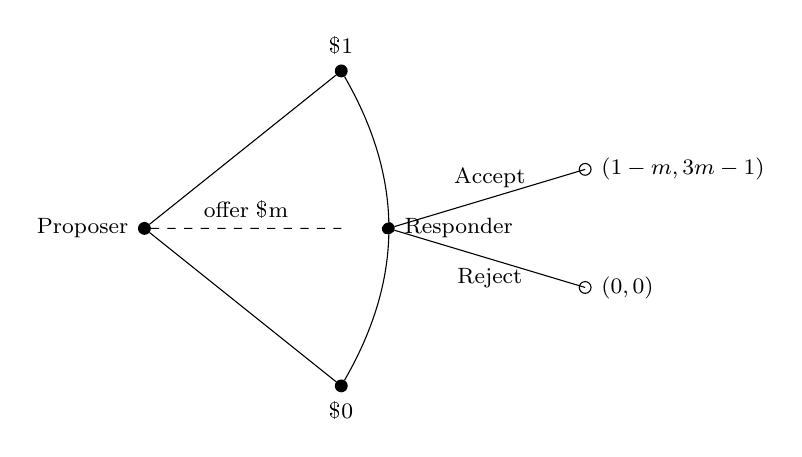
\begin{tikzpicture}[font=\footnotesize,
                    grow' = right
                    ]
\tikzstyle{level 1}=[level distance=25mm, sibling distance=20mm]
\tikzstyle{level 2}=[level distance=25mm, sibling distance=15mm]

    \node(0)[solid node, label=left:{Proposer}]{}
        % Upper part of arc
        child{node[solid node, label=above:{\$1}]{}}
        % Where y is chosen/offered, general case
        child{[dashed] node[solid node, xshift=17, label=right:{Responder}]{}
            child{[solid, black] node[hollow node, label=right:{$(1-m, 3m-1)$}]{} edge from parent node[above]{Accept}}
            child{[solid, black] node[hollow node, label=right:{$(0,0)$}]{} edge from parent node[below]{Reject}}
            edge from parent node[above]{\textcolor{black}{offer \$m}}
        }
        child{node[solid node, label=below:{\$0}]{}}
    ;

    \draw[bend left](0-1)to(0-3);


\end{tikzpicture}
\end{center}

\item Find and report the subgame perfect equilibrium. Note how equilibrium behavior depends on $a$.
$$(3m-1) \geq 0 $$
$$m \geq \frac{1}{3} $$

SPNE: (Offer $\$\frac{1}{3}$, accept)

\end{enumerate}

\end{document}
